\documentclass{beamer}
\usepackage[english, russian]{babel}
\usepackage[T2A]{fontenc}
\usepackage[utf8]{inputenc}
\usepackage{indentfirst}
\usepackage{amsmath, amsfonts, amssymb, amsthm, mathtools}
\usepackage[export]{adjustbox}
\usepackage{graphicx} 
\graphicspath{ {./images/} }

\usepackage{subcaption}
\usepackage{verbatim}

\usepackage{minted}{\setlength{\parskip}{0pt}}

\usepackage{hyperref}

\hypersetup{
    colorlinks=true,
    linkcolor=blue,
    filecolor=magenta,      
    urlcolor=black,
    pdftitle={Overleaf Example},
    pdfpagemode=FullScreen,
    }


\title{Лабораторная работа № 10. \\Расширенные настройки SMTP-сервера}
\author{Данила Стариков \\ НПИбд-02-22}
\institute{Российский университет дружбы народов имени Патриса Лумумбы}
\date{2024}

\begin{document}

\frame{\titlepage}

\begin{frame}
\frametitle{Цель работы}
\begin{itemize}
    \item Приобретение практических навыков по конфигурированию SMTP-сервера в части настройки аутентификации
\end{itemize}
\end{frame}

\begin{frame}
  \frametitle{Настройка LMTP в Dovecote}
  \centering
  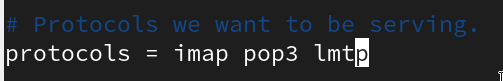
\includegraphics[width=\textwidth]{../images/image01.png}
  \captionof{figure}{Обновление списка разрешенных протоколов в Dovecot.}  
\end{frame}

\begin{frame}
  \frametitle{Настройка LMTP в Dovecote}
  \centering
  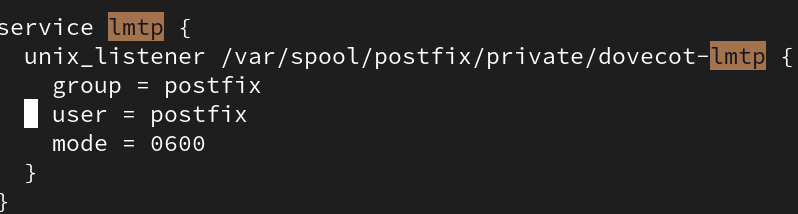
\includegraphics[width=\textwidth]{../images/image02.png}
  \captionof{figure}{Настройки сервера \texttt{lmtp}.}
\end{frame}

\begin{frame}
  \frametitle{Настройка LMTP в Dovecote}
  \centering
  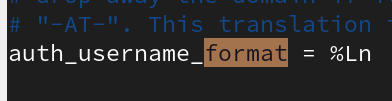
\includegraphics[width=\textwidth]{../images/image03.png}
  \captionof{figure}{Задание формата имени пользователя для аутентификации.}
\end{frame}

\begin{frame}
  \frametitle{Настройка LMTP в Dovecote}
  \centering
  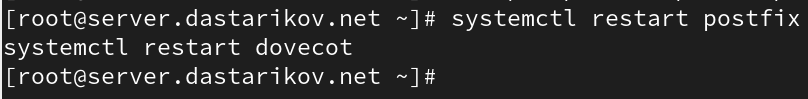
\includegraphics[width=\textwidth]{../images/image04.png}
  \captionof{figure}{Перезагрузка Postfix и Dovecot.}  
\end{frame}

\begin{frame}
  \frametitle{Настройка LMTP в Dovecote}
  \centering
  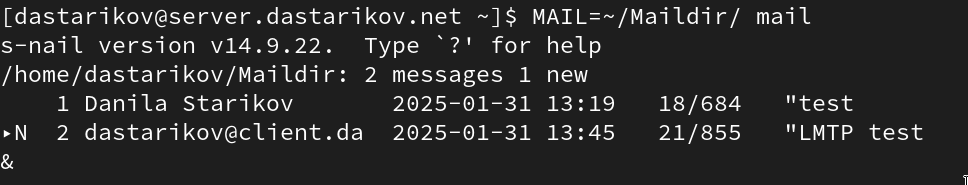
\includegraphics[width=\textwidth]{../images/image05.png}
  \captionof{figure}{Просмотр доставленного письма через утилиту \texttt{mail}.}
\end{frame}

\begin{frame}
  \frametitle{Настройка LMTP в Dovecote}
  \centering
  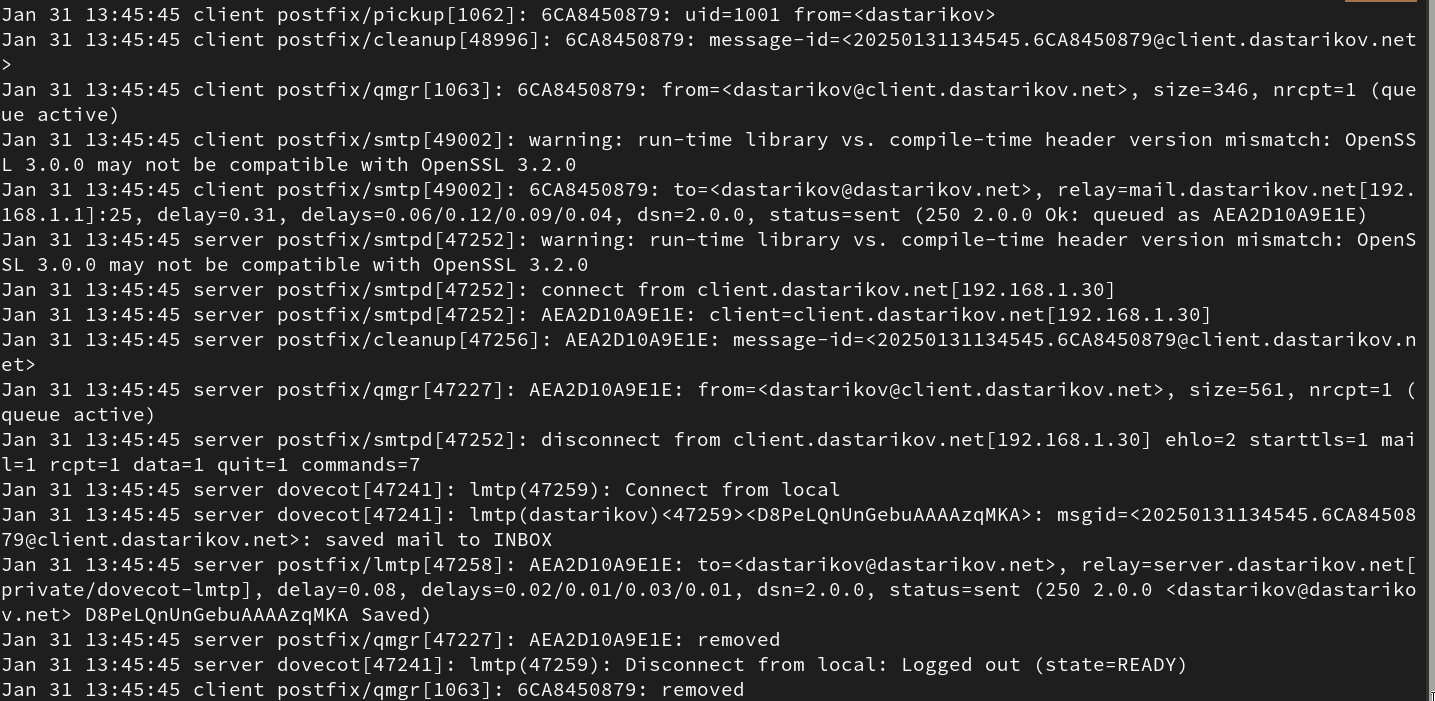
\includegraphics[width=\textwidth]{../images/image06.png}
  \captionof{figure}{Просмотр логов при отправке письма.}
\end{frame}

\begin{frame}
  \frametitle{Настройка SMTP-аутентификации} 
  \centering
  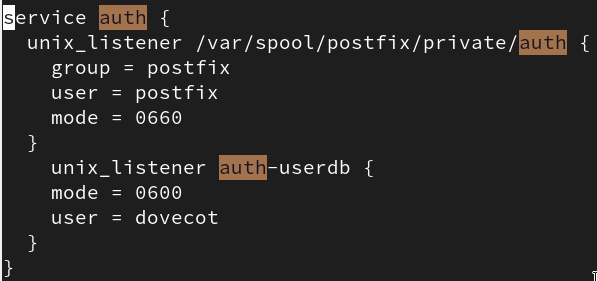
\includegraphics[width=\textwidth]{../images/image08.png}
  \captionof{figure}{Настройка службы аутентификации.} 
\end{frame}

\begin{frame}
  \frametitle{Настройка SMTP-аутентификации}
  \centering
  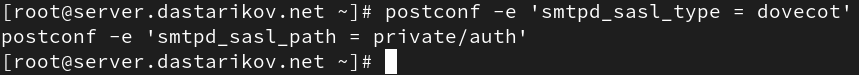
\includegraphics[width=\textwidth]{../images/image09.png}
  \captionof{figure}{Настройка типа аутентификации SASL для \texttt{smtpd}.}  
\end{frame}

\begin{frame}
  \frametitle{Настройка SMTP-аутентификации}
  \centering
  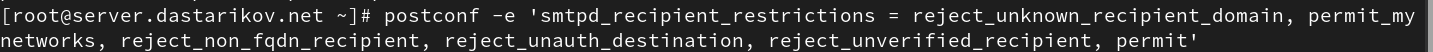
\includegraphics[width=\textwidth]{../images/image10.png}
  \captionof{figure}{Настройка Postfix для запрета спамрассылок.}
\end{frame}

\begin{frame}
  \frametitle{Настройка SMTP-аутентификации}
  \centering
  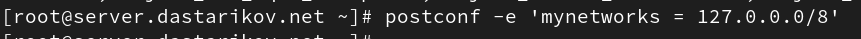
\includegraphics[width=\textwidth]{../images/image11.png}
  \captionof{figure}{Ограничение приема почты только локальным адресом.}
\end{frame}

\begin{frame}
  \frametitle{Настройка SMTP-аутентификации}
  \centering
  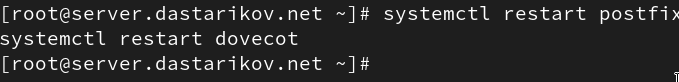
\includegraphics[width=\textwidth]{../images/image13.png}
  \captionof{figure}{Перезагрузка Postfix и Dovecot.}
  \label{13}
\end{frame}

\begin{frame}
  \frametitle{Настройка SMTP-аутентификации}
  \centering
  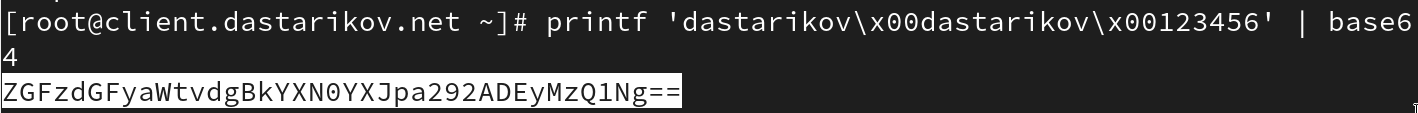
\includegraphics[width=\textwidth]{../images/image14.png}
  \captionof{figure}{Получение строки для аутентификации.}  
\end{frame}

\begin{frame}
  \frametitle{Настройка SMTP-аутентификации}
  \centering
  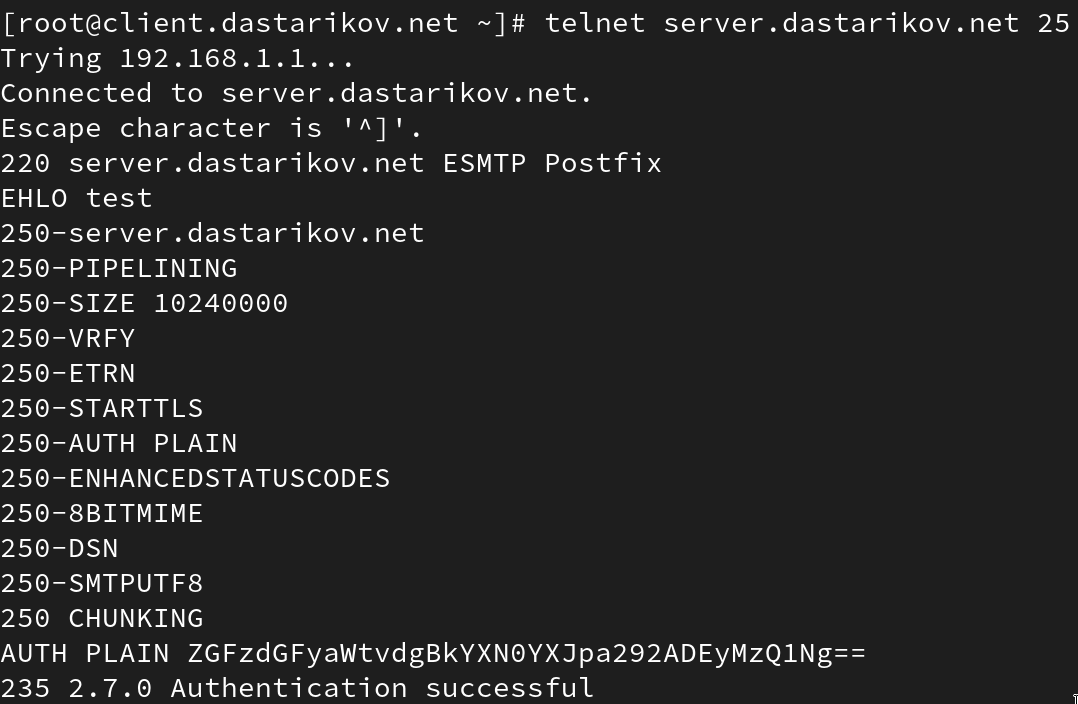
\includegraphics[width=\textwidth]{../images/image15.png}
  \captionof{figure}{Подключение к SMTP-серверу через \texttt{telnet}.}
\end{frame}


\begin{frame}
  \frametitle{Настройка SMTP over TLS}
    \centering
    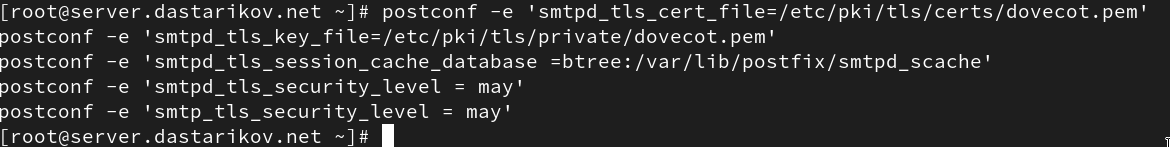
\includegraphics[width=\textwidth]{../images/image16.png}
    \captionof{figure}{Конфигурация Postfix для работы через TLS.}  
\end{frame}

\begin{frame}
  \frametitle{Настройка SMTP over TLS}
      \centering
    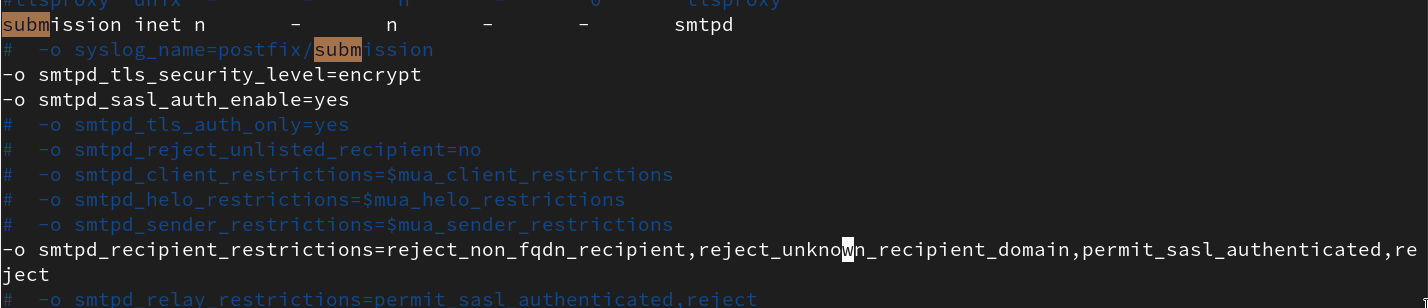
\includegraphics[width=\textwidth]{../images/image17.png}
    \captionof{figure}{Изменение \texttt{/etc/postfix/master/cf}.}
\end{frame}

\begin{frame}
  \frametitle{Настройка SMTP over TLS}
    \centering
    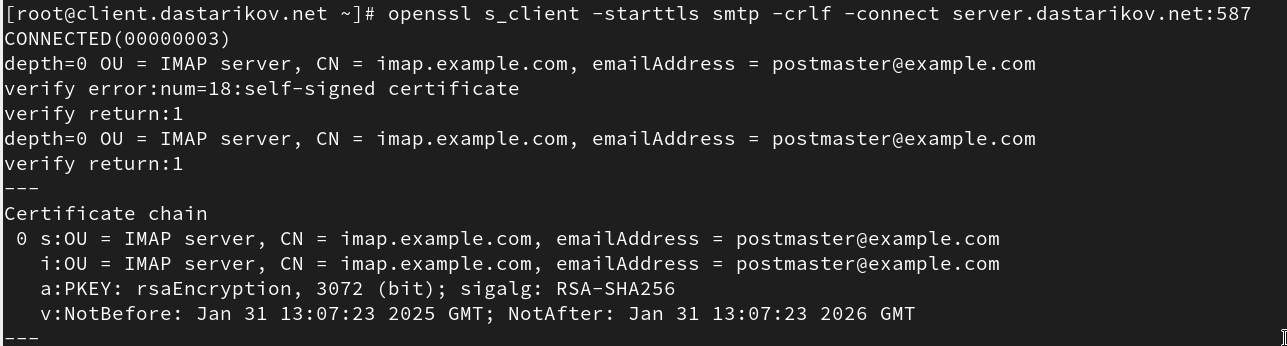
\includegraphics[width=\textwidth]{../images/image18.png}
    \captionof{figure}{Подключение к SMTP-серверу через \texttt{openssl}.}  
\end{frame}

\begin{frame}
  \frametitle{Настройка SMTP over TLS}
    \centering
    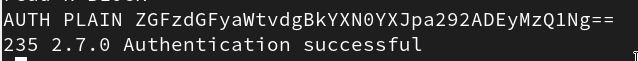
\includegraphics[width=\textwidth]{../images/image19.png}
    \captionof{figure}{Проверка подключения к SMTP-серверу через \texttt{telnet}.}  
\end{frame}

\begin{frame}
  \frametitle{Настройка SMTP over TLS}
    \centering
    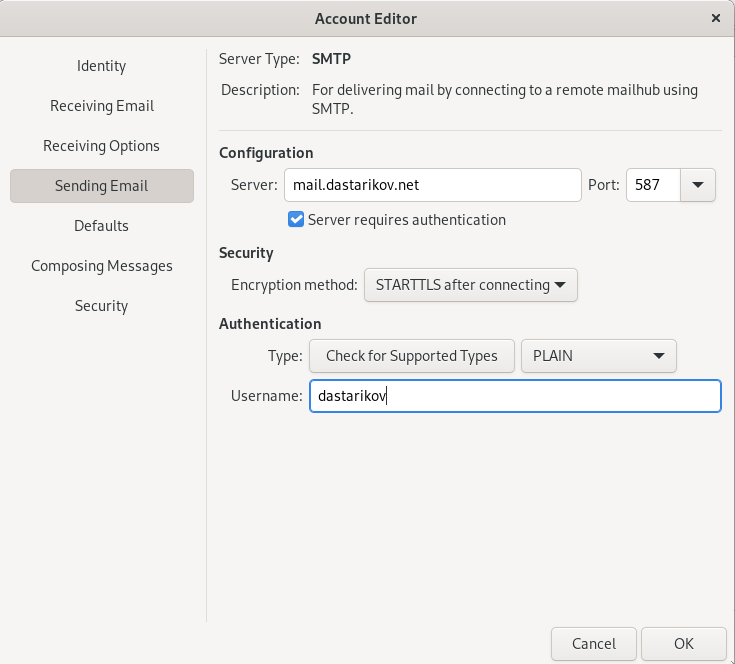
\includegraphics[width=0.8\textwidth]{../images/image20.png}
    \captionof{figure}{Корректировка почтового клиента Evolution.}  
\end{frame}

\begin{frame}
  \frametitle{Настройка SMTP over TLS}
    \centering
    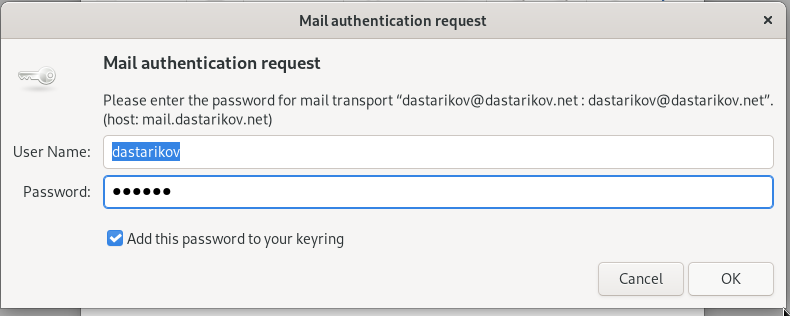
\includegraphics[width=\textwidth]{../images/image21.png}
    \captionof{figure}{Аутентификация пользователя при попытке отправить письмо.}  
\end{frame}

\begin{frame}
  \frametitle{Настройка SMTP over TLS} 
    \centering
    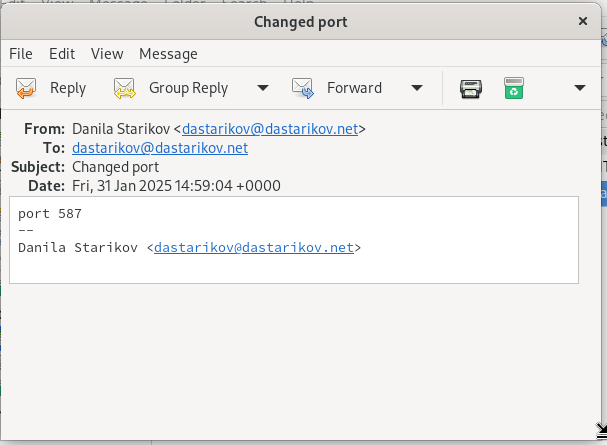
\includegraphics[width=\textwidth]{../images/image22.png}
    \captionof{figure}{Просмотр пришедшего письма.} 
\end{frame}

\begin{frame}[fragile]
  \frametitle{Внесение изменений в настройки внутреннего окружения виртуальной машины}
    \begin{minted}[breaklines]{bash}
    cd /vagrant/provision/server
    cp -R /etc/dovecot/dovecot.conf /vagrant/provision/server/mail/etc/dovecot/
    cp -R /etc/dovecot/conf.d/10-master.conf /vagrant/provision/server/mail/etc/dovecot/conf.d/
    cp -R /etc/dovecot/conf.d/10-auth.conf /vagrant/provision/server/mail/etc/dovecot/conf.d/
    mkdir -p /vagrant/provision/server/mail/etc/postfix/
    cp -R /etc/postfix/master.cf /vagrant/provision/server/mail/etc/postfix/
  \end{minted}
  \begin{itemize}
  \item Внесли изменения в \texttt{mail.sh} по расширенной конфигурации SMTP-сервера
  \item На клиенте добавили установку \texttt{Telnet}
  \end{itemize}
\end{frame}

\begin{frame}
\frametitle{Выводы}
\begin{itemize}
    \item В результате выполнения лабораторной работы приобрели практические навыки по конфигурированию SMTP-сервера в части настройки аутентификации.
\end{itemize}
\end{frame}
\end{document}
